\documentclass[10pt,pdf,utf8,english,compress,hyperref={unicode}]{beamer}
\usepackage{ifxetex}
\usepackage[english]{babel}
\ifxetex
\else
\usepackage[utf8]{inputenc}
\usepackage[T2A]{fontenc}
\usepackage[backend=biber,style=authoryear]{biblatex}
\fi
\usepackage{booktabs}
\usepackage[scale=2]{ccicons}
\usepackage{url}
\usepackage{listings}
\usepackage{booktabs}
\usepackage{hyperref}
\usepackage{drawstack}
\usepackage{animate}
\usepackage{tikz}
\usepackage[normalem]{ulem}
\usetikzlibrary{shapes,arrows}

\graphicspath{{./pix/}}
%\usetheme[useTitleProgressBar]{m}
\usetheme{m}

% ------ Embed URL in the reference title ------

\ifxetex
% ---- START
\else
\renewbibmacro*{url+urldate}{}

\newbibmacro{string+doiurl}[1]{%
	\iffieldundef{doi}{%
		\iffieldundef{url}{%
			#1%
		}{%
			\href{\thefield{url}}{#1}%
		}%
	}{%
		\href{http://dx.doi.org/\thefield{doi}}{#1}%
	}%
}

\DeclareFieldFormat{title}{\usebibmacro{string+doiurl}{\mkbibemph{#1}}}
\DeclareFieldFormat[article,incollection]{title}{\usebibmacro{string+doiurl}{\mkbibemph{#1}}}

% ------ Nice and shiny bibliography list -------

\setbeamertemplate{bibliography item}{%
	\ifboolexpr{test {\ifentrytype{book}} or test {\ifentrytype{mvbook}}
	or test {\ifentrytype{collection}} or test {\ifentrytype{mvcollection}}
	or test {\ifentrytype{reference}} or test {\ifentrytype{mvreference}} }
	{\setbeamertemplate{bibliography item}[book]}
	{\ifentrytype{online}
		{\setbeamertemplate{bibliography item}[online]}
		{\setbeamertemplate{bibliography item}[article]}}%
	\usebeamertemplate{bibliography item}}

\defbibenvironment{bibliography}
	{\list{}
		{\settowidth{\labelwidth}{\usebeamertemplate{bibliography item}}%
		\setlength{\leftmargin}{\labelwidth}%
		\setlength{\labelsep}{\biblabelsep}%
		\addtolength{\leftmargin}{\labelsep}%
		\setlength{\itemsep}{\bibitemsep}%
		\setlength{\parsep}{\bibparsep}}}
	{\endlist}
	{\item}
% ----- END
\fi

% ------ Document starting here -------

\title{Radare2 as a tool for CTF}
\subtitle{Basic reference}
\author{Anton Kochkov (@akochkov)}
\date{\today}
\institute{KeenLab of Tencent, TCTF 2017}

\ifxetex
\else
\addbibresource{refs.bib}
% Just a hack to workaround 'Package keyvar error: langjapanese undefined'
% Will be fixed in biblatex 3.2 and biber 2.3
% See more at:
% https://tex.stackexchange.com/questions/277314/package-keyval-error-langjapanese-undefined
\NewBibliographyString{langjapanese}
\NewBibliographyString{fromjapanese}
\fi

% ------------------------------------------------------------------------------------
\begin{document}
\maketitle

% ------------------------------------------------------------------------------------
\section{Introduction}

\begin{frame}[fragile]
  \frametitle{History}
  \begin{itemize}
	  \item Incepted in 2006 by Sergi Alvarez aka Pancake (@trufae) as Radare1
	  \item Initially designed as a forensic tool
	  \item Rewritten from scratch in 2009 for modular architecture
	  \item Scriptable and extendable framework, not just a tool
	  \item Gained popularity only a few years ago
	  \item Participation in GSoC\footfullcite{r2gsoc2017} and institutioning own
	  RSoC\footfullcite{r2rsoc2017}
  \end{itemize}
\end{frame}

\begin{frame}[fragile]
  \frametitle{Short overview}
  \begin{itemize}
	\item Core part written in the pure C without dependencies
	\item Highly portable to different platforms
	\item UNIX (KISS) -like tools
	\item Around 1000 commands
	\item More than 400 configuration options
	\item Supports both static and dynamic analysis
	\item Own package manager and external plugins infrastructure
	\item Windows support from the box (and GSoC task)
  \end{itemize}
\end{frame}

\begin{frame}[fragile]
  \frametitle{Installation}
  \begin{itemize}
	  \item First rule - don't use packaged version
	  \item \alert{sys/install.sh} on *nix, including OS X
	  \item prebuilt EXE on Windows (best in ConEmu)
	  \item Current release version is \textbf{1.5.0}
	  \item Debian (and Ubuntu?) still ship \textbf{0.9.6}
	  \item Use version from git for bug-reporting
  \end{itemize}
\end{frame}

\begin{frame}[fragile]
  \frametitle{Toolset review}
  \begin{itemize}
	\item \textbf{Radare2} - the main tool, incorporate everything
	\item \textbf{Rabin2} - parsing binaries
	\item \textbf{Radiff2} - diffing binaries
	\item \textbf{Rafind2} - searching
	\item \textbf{Ragg2} - writing shellcodes
	\item \textbf{Rahash2} - calculating hashes
	\item \textbf{Rarun2} - setting up running environment
	\item \textbf{Rasm2} - CLI assembler/disassembler
  \end{itemize}
\end{frame}

\section{Short cheatsheet}

\begin{frame}[fragile]
  \frametitle{Commands concept}
  \begin{itemize}
  % TODO: add a reference to ``Migration from GDB'
	  \item Most of the commands are abbreviations
	  \item Similar as in GDB (\textbf{info registers} -> \textbf{i r}) but w/o space\footfullcite{r2gdbmigration}
	  \item See registers - \alert{dr} (Debug), \alert{aer} (ESIL)
	  \item \alert{dr} == debug register
	  \item \alert{aer} == analysis ESIL register
	  \item Each command has internal help - just add \textbf{'?'}
	  \item Most of the commands has JSON output - just add \textbf{'j'}
	  \item Case sensitive (see commands' count)
  \end{itemize}
\end{frame}

\begin{frame}[fragile]
  \frametitle{Basic disassembly\footfullcite{r2bookdisasm}}
  \begin{itemize}
	  \item \textbf{rasm2 -a arm -b 64 -d 058d00f8}
	  \item \textbf{rasm2 -a arm "mov r0, 5"}
	  \item \alert{pd [N]} - linear disassembly of [N] insturctions
	  \item \alert{pi [N]} - the same, just instructions
  \end{itemize}
	  Those 3 below require functions defined first (analysis)
  \begin{itemize}
	  \item \alert{pdf [function name]} - linear disassembly of function
	  \item \alert{pdr} - recursive disassembly across function graph
	  \item \alert{pdc} - basic \textbf{C-like} pseudocode
  \end{itemize}
\end{frame}

\begin{frame}[fragile]
  \frametitle{Basic debug\footfullcite{r2bookdebug}}
  \begin{itemize}
	  \item Add \textbf{"-d"} option to radare2
	  \item Or reopen it using \alert{ood} command
	  \item \textbf{r2 -d /bin/ls}
  \end{itemize}
  Debug commands are under \textbf{"d"} namespace - see \alert{d?}
  \begin{itemize}
	  \item \alert{db} - Setting breakpoint
	  \item \alert{dc} - Continuing execution
	  \item \alert{ds} - Single step
	  \item \alert{ds [address]} - Step until
	  \item Functional keys in visual mode, see \alert{V?}
  \end{itemize}
\end{frame}

\begin{frame}[fragile]
	\frametitle{Visual debug}
	\begin{figure}
		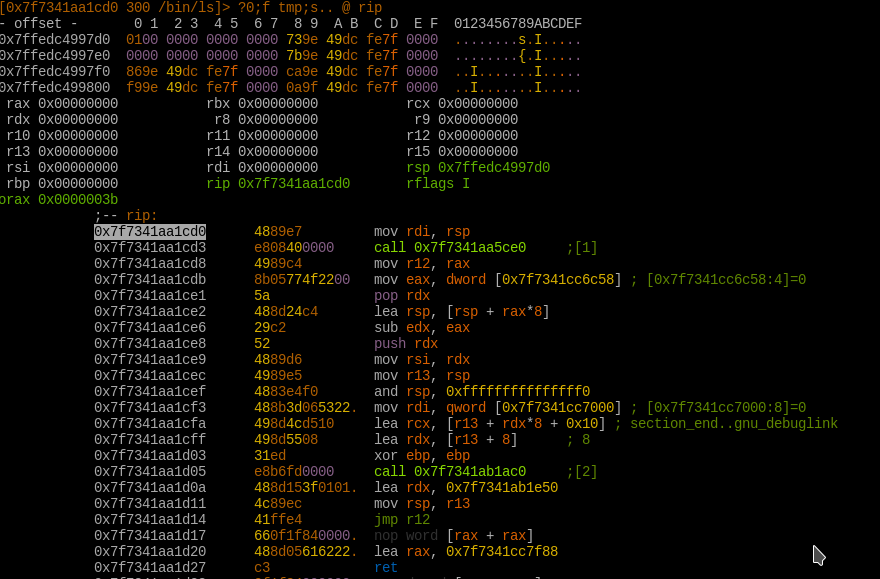
\includegraphics[width=\linewidth]{r2visualdebug.png}
	\end{figure}
\end{frame}

\begin{frame}[fragile]
  \frametitle{Basic patching\footfullcite{r2bookwrite}}
  There are many searching options (see \alert{/?} output),
  including ROP gadgets search (\alert{/R})
  \begin{itemize}
	  \item Add \textbf{"-w"} option to radare2 to open in write mode
	  \item Or reopen it using \alert{oo+} command
  \end{itemize}
  Writing commands are under \textbf{"w"} namespace - see \alert{w?}
  \begin{itemize}
	  \item \alert{w} - Write ASCII string
	  \item \alert{wx} - Write hexadecimal sequence
	  \item \alert{wa} - Write assembly
	  \item \alert{wtf} - Write to file
  \end{itemize}
\end{frame}

\begin{frame}[fragile]
  \frametitle{Visual modes}
  \begin{itemize}
	  \item Can use UTF-8 and True color % reference to UTF-8 and TrueColor
	  \item \alert{e scr.utf8=true ; e scr.truecolor=true}
	  \item All visual modes are under \textbf{"V"} namespace
	  \item Just press \textbf{V} and loop forward/back using \textbf{p/P}
	  \item \alert{VV} - ASCII graphs
	  \item \alert{V\_} - HUD mode
	  \item \alert{VF} - navigation through flags/symbols (supports p/P too)
	  \item \alert{Ve} - navigation (and preview) of internal config variables
	  \item \alert{Vt} - navigation through types
	  \item Has different hotkeys - see \alert{V?}
	% reference to visual section in the book
  \end{itemize}
\end{frame}

\begin{frame}[fragile]
	\frametitle{Ve - visual config}
	\begin{figure}
		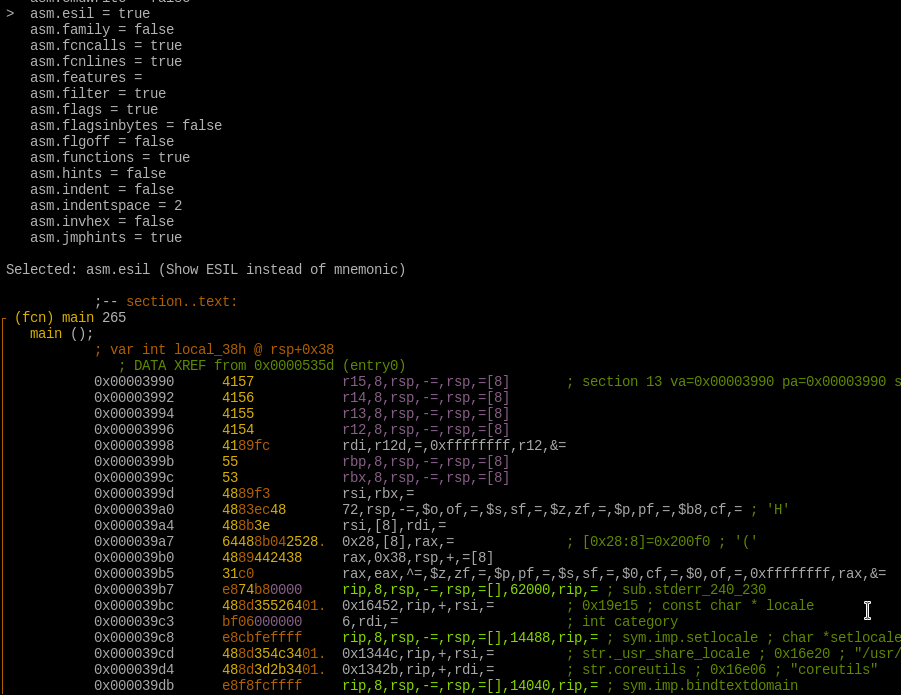
\includegraphics[width=\linewidth]{r2visualconfig.png}
	\end{figure}
\end{frame}

\begin{frame}[fragile]
	\frametitle{VF - visual flagspaces}
	\begin{figure}
		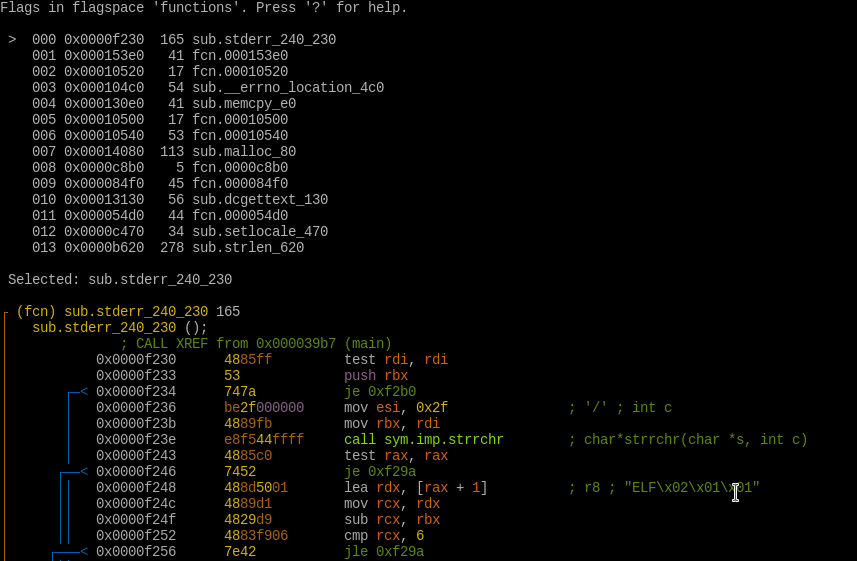
\includegraphics[width=\linewidth]{r2visualflagspace.png}
	\end{figure}
\end{frame}

\section{Analysis}

\begin{frame}[fragile]
  \frametitle{Analysis options}
  \begin{itemize}
	  \item Located in \textbf{e anal.*} config var namespace
	  \item For example enabling jump tables analysis \alert{e anal.jmptbl=true}
	  \item We don't enable all analysis by default
	  \item \textbf{r2 -A /bin/ls} - open with autoanalysis
	  \item \textbf{r2 -e bin.demangle=true /bin/ls} - open with demangling
	  \item \alert{e asm.demangle=true} - show demangled symbols in disassembly
	  \item \alert{e pdb.} - options related to loading/downloading PDBs
	  \item \alert{e asm.} - options to control information shown in disasm
	% reference to analysis section of the book
	% reference to the asciinema?
  \end{itemize}
\end{frame}

\begin{frame}[fragile]
  \frametitle{Analysis commands}
  \begin{itemize}
	  \item There are a few autoanalysis commands: aa, aaa and aaaa
	  \item Those offer different analysis depth
	  \item All analysis commands are under \textbf{"a"} namespace - see \alert{a?}
	  \item \textbf{r2 -A}, \textbf{r2 -AA},.. - same with options
	  \item \alert{af} - analyze the function (see also \alert{af?})
	  \item \alert{av} - show virtual tables (C++)
	  \item \alert{aa?} - particular commands for recursive analysis
	  \item \alert{aac} - analyze function calls
	  \item \alert{aad} - analyze data references
	  \item \alert{ax?} - particular commands for analyzing references (e.g. \alert{axt})
	% reference to analysis section of the book
	% reference to the asciinema?
  \end{itemize}
\end{frame}

\begin{frame}[fragile]
	\frametitle{ASCII graph}
	\begin{figure}
		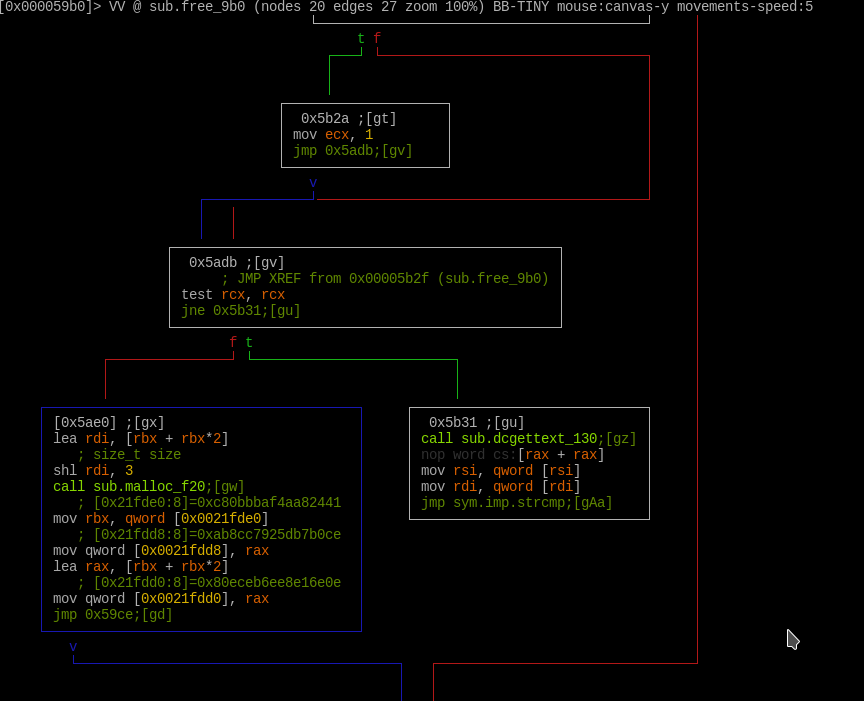
\includegraphics[width=\linewidth]{r2asciigraph.png}
	\end{figure}
\end{frame}

\begin{frame}[fragile]
  \frametitle{ASCII/Unicode graphs}
  \begin{itemize}
	  \item After analysis is done graph information is available
	  \item \alert{agC} - generate Graphviz code
	  \item \alert{agf} - show ASCII graph of the function
	  \item \alert{VV} - visual ASCII graph
	  \item It's possible to navigate through nodes using \textbf{Tab/Shift+Tab}
	  \item There is support for \textbf{"zoom"} - \textbf{+/-}
	  \item Minimap support - press \textbf{p/P} to scroll via all modes
	  \item Also graphs information available via JSON (for WebUI)
	% reference to visual graphs of the book
	% reference to the asciinema?
  \end{itemize}
\end{frame}

\begin{frame}[fragile]
	\frametitle{Minimap}
	\begin{figure}
		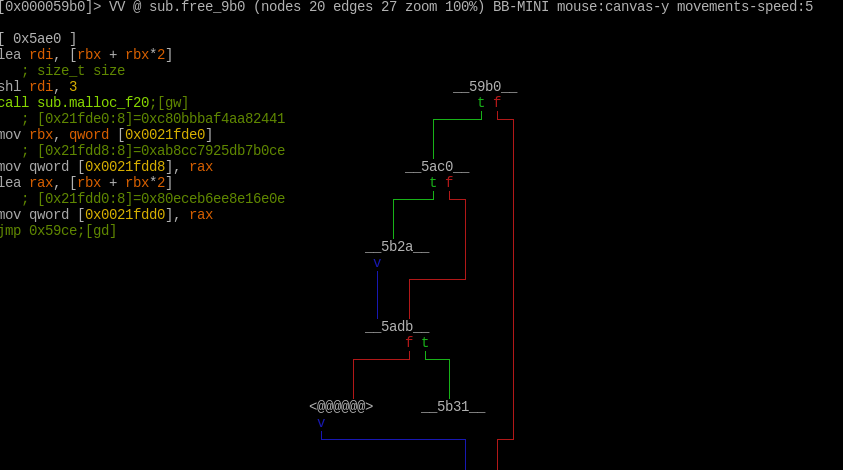
\includegraphics[width=\linewidth]{r2minimap.png}
	\end{figure}
\end{frame}

\begin{frame}[fragile]
  \frametitle{Types}
  \begin{itemize}
	  \item There is a support for C types
	  \item All types commands are located in \textbf{``t''} namespace - see \alert{t?}
	  \item \alert{to file.h} - parse C header file and load types from it
	  \item \alert{td struct qwe \{int a; char* b;\};} - parse type desc
	  \item \alert{tp <typename> = <address>} - cast data at some addr to type
	  \item \alert{tl <typename> = <address>} - permanently link type to addr
	  \item \alert{tk} - raw requests to SDB database (types storage)
	  \item \alert{Vt} - visual types navigation
	% reference to visual graphs of the book
	% reference to the asciinema?
  \end{itemize}
\end{frame}

\begin{frame}[fragile]
  \frametitle{Arguments}
  \begin{itemize}
	  \item There is a support for function arguments
	  \item All arguments commands are located in \textbf{``afv''} namespace - see \alert{afv?}
	  \item \alert{afv} - show locals/arguments
	  \item \alert{afvn} - rename argument/local
	  \item \alert{afvr?} - manipulation of register based arguments
	  \item \alert{afvs?} - manipulation of SP based arguments
	  \item \alert{afvb?} - manipulation of BP based arguments
	  \item \alert{afta} - analyze all arguments + types across file
	% reference to arguments/locals of the book
	% reference to the asciinema?
  \end{itemize}
\end{frame}

\begin{frame}[fragile]
  \frametitle{ESIL\footfullcite{r2esil}}
  \begin{itemize}
	  \item R2 has its own Intermediate Language and its VM
	  \item It's RPN form (Reverse Polish Notation)\footfullcite{r2esil-instruction-set}
	  \item Allows to emulate parts of the programs
	  \item Supported architectures are x86, ARM, MIPS, etc...
	  \item Being used in the deep analysis for resolving indirect jumps
	  \item \alert{ao~esil} - shows the ESIL representation of current instruction
	  \item \alert{ae eax,5,+=} - evaluate ESIL expression
	  \item \alert{e asm.esil=true} - show ESIL instead of disassembly
	% reference to the asciinema?
  \end{itemize}
\end{frame}

% TODO: put some DEMO here?

\begin{frame}[fragile]
  \frametitle{Memory inspection}
  For this R2 need to be started in debug mode (\textbf{``-d''})
  \begin{itemize}
	  \item \alert{dm?} commands allows you to inspect the memory
	  \item \alert{dmm} - shows loaded libraries
	  \item \alert{dm} - inspecting the memory map
	  \item \alert{dmh?} - commands to inspect the heap
	  \item \alert{dmhg} - show the ASCII graph of the heap
	  \item \alert{dmhb} - display parsed bins for selected heap arena
	  \item \alert{dbta} - show the ASCII graph of call stack
	% reference to heap documentation
	% reference to heap exploitation
	% reference to the asciinema?
  \end{itemize}
\end{frame}

\begin{frame}[fragile]
	\frametitle{Stack visualization}
	\begin{figure}
		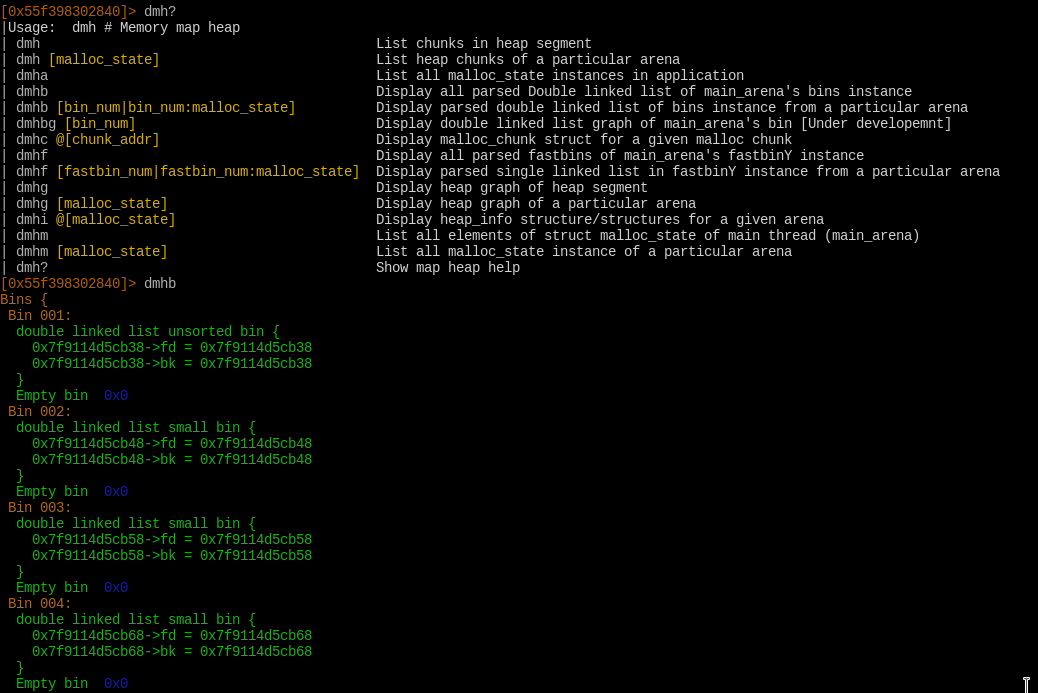
\includegraphics[width=\linewidth]{r2heapbins.png}
	\end{figure}
\end{frame}

\begin{frame}[fragile]
	\frametitle{Stack visualization}
	\begin{figure}
		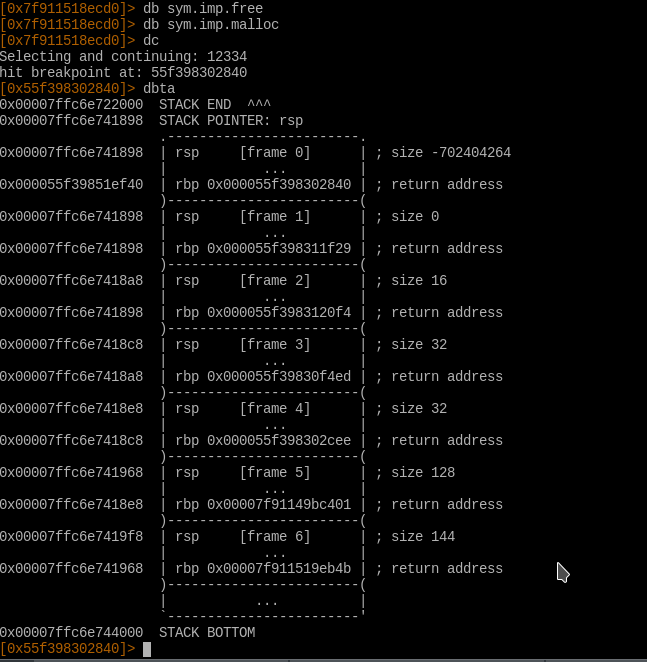
\includegraphics[width=\linewidth]{r2visualstack.png}
	\end{figure}
\end{frame}

% TODO: put some DEMO here?
\section{Debugging}

\begin{frame}[fragile]
  \frametitle{Native debugging}
  \begin{itemize}
	  \item For this R2 need to be started in debug mode (\textbf{"-d"} option)
	  \item Or reopen using \alert{ood}
	  \item \alert{dr=} to show the registers
	  \item \alert{dbt} - display backtrace
	  \item \alert{dt?} - tracing features
	  \item \alert{dp?} - listing/attaching/etc to processes
	  \item \alert{dk?} - working with signals
	% reference to debug documentation documentation
	% reference to the asciinema?
  \end{itemize}
\end{frame}

% TODO: put some DEMO here?

\begin{frame}[fragile]
\frametitle{GDB Remote connection}
\begin{itemize}
	\item Just connect using \textbf{gdb://} protocol
	\item \textbf{gdbserver /bin/ls}
	\item \textbf{r2 -D gdb gdb://localhost:1234}
	\item Support the same commands as other debug engines
	\item Can be used to connect GDBserver of QEMU, VMWare, etc
	\item This year our GSoC student also working on improving\footfullcite{r2gsoc2017ideasgdb}
	\item And also working on small gdbserver implementation
  % reference to GDB remote protocol documentation
  % reference to the asciinema?
\end{itemize}
\end{frame}

\begin{frame}[fragile]
\frametitle{WinDbg Remote connection}
\begin{itemize}
	\item Just connect using \textbf{windbg://} protocol
	\item Run VBox or QEMU with Windows debug over pipes
	\item \textbf{r2 -D wind windbg:///tmp/windbg.pipe}
	\item Support the same commands as other debug engines
	\item This year another GSoC student also working on improving
	this\footfullcite{r2gsoc2017ideaswindows}
	\item For now it supports only connection via serial (pipe) - no network
	\item Our own WinDbg protocol parser\footfullcite{r2windbg} - can be reused in other projects
  % reference to the asciinema?
\end{itemize}
\end{frame}

\begin{frame}[fragile]
\frametitle{Integration with FRIDA\footfullcite{frida}}
\begin{itemize}
	\item Just install Frida and r2frida\footfullcite{r2frida} (\textbf{r2pm -i r2frida})
	\item \textbf{r2 frida://<phone\_id>/Appname}
	\item r2frida implements IO layer smoothly redirecting commands
  % reference to the asciinema?
\end{itemize}
\end{frame}

\begin{frame}[fragile]
  \frametitle{ESIL\footfullcite{r2esil} debugging}
  \begin{itemize}
	  \item \alert{aei} - initialize ESIL VM
	  \item \alert{aeim} - initialise memory for selected parameters
	  \item \alert{aeip} - point ESIL VM to current IP
	  \item \alert{aer eax=0x5} - set register value
	  \item \alert{aes} - step using ESIL emulation
	  \item \alert{aecu} - continue until using ESIL emulation
	  \item Also stepping using ESIL is available in visual debug mode
	% reference to ESIL chapters in the book
	% reference to the asciinema?
  \end{itemize}
\end{frame}

% TODO: Image of ESIL

\begin{frame}[fragile]
  \frametitle{Timeless debug}
  R2 supports basic timeless debug. Moreover, this year GSoC\footfullcite{r2gsoc2017blog} student working on improving it.
  \begin{itemize}
	  \item \alert{dts+} - add the trace session
	  \item \alert{dts} - show the active trace sessions
	  \item \alert{dms?} - work with memory snapshots
	  \item \alert{dsb} - single step back
	% reference to the asciinema?
  \end{itemize}
\end{frame}

\section{Signatures}

\begin{frame}[fragile]
  \frametitle{Native signatures}
  Radare2 has different searching capabilities\footfullcite{r2booksearch} including signatures:
  \begin{itemize}
	  \item \alert{z} - show signatures status and \alert{z*} to list them
	  \item \alert{zb} - define signature in place
	  \item \alert{zo} - manage signature files
	  \item \alert{zos} - save the signature into file
	  \item \alert{z/} - search signatures
	  \item \alert{zs} - manage singature spaces
	% reference to signatures section of the book
	% reference to the asciinema?
  \end{itemize}
\end{frame}

\begin{frame}[fragile]
  \frametitle{FLIRT and Yara}
  \begin{itemize}
  % TODO: Add links to FLIRT format and Yara site
	  \item R2 has support for loading FLIRT signatures (IDA < 6.8)
	  \item \alert{zfs} - load FLIRT signature from the file and scan
	  \item \alert{zfd} - dump the contents of the FLIRT file
	  \item \alert{zfz} - convert FLIRT file to native signature format
  \end{itemize}
  R2 can support Yara via plugin: \textbf{r2pm -i yara-lib; r2pm -i yara}
  \begin{itemize}
	  \item \alert{yara add} - load Yara rules from the file
	  \item \alert{yara scan} - to scan the file for matches
	  \item \alert{yara list} - show loaded Yara signatures
	  \item \alert{yara clear} - clear all loaded rules
	% reference to analysis section of the book
	% reference to the asciinema?
  \end{itemize}
\end{frame}

\section{Scripting}

\begin{frame}[fragile]
  \frametitle{Internal scripting\footfullcite{r2bookscript}}
  \begin{itemize}
	  \item R2 has variables - see \alert{?\$?} output
	  \item R2 supports iterators - see \alert{?@?} output
	  \item \alert{pd 1; ao 1} - sequence the commands
	  \item \alert{ao | grep esil} - pipe into external commands
	  \item \alert{\#! tcpdump} - run system command
	  \item \alert{px 10 @ `ao~ptr[1]`} - like shell backtick
	  \item Redirecting output using \alert{>} and \alert{>>}
	% reference to the asciinema?
  \end{itemize}
\end{frame}

\begin{frame}[fragile]
  \frametitle{Loops, macroses and aliases}
  \begin{itemize}
	  \item \alert{afi @@ fcn.* ~name} - grep through output of afi of matching
	  \item \alert{ao @@=\$\$ \$\$2} - looping over cur offset and cur offset +2
	  \item \alert{pi 1 @@i} - looping over instructions in the funtion
	  \item \alert{afi @@@ functions ~name[1]} - looping over functions
	  \item \alert{(qwe, pd4, ao)} - add macro \textbf{``qwe''}, call with \alert{.(qwe)}
	  \item \alert{(foo x y, pd \$0; s +\$1)} - macro with arguments
	  \item \alert{\$<aliasname>=<command>} - define an alias
	  \item \alert{\$dis='pi 1;ao'}, then call \alert{\$dis}
	% reference to the asciinema?
  \end{itemize}
\end{frame}

\begin{frame}[fragile]
  \frametitle{r2pipe}
  \begin{itemize}
	  \item R2 has a mechanism for interacting with scripts via pipe\footfullcite{r2pipe}
	  \item \textbf{pip install r2pipe}, \textbf{npm install r2pipe}
	  \item In python just do \textbf{import r2pipe} and use provided commands
	  \item Python r2pipe scripts can be run from internal shell
	  \item \alert{. myscript.py} - just use source command \alert{.}
	% reference to an r2pipe example
	% reference to the asciinema?
  \end{itemize}
\end{frame}

\begin{frame}[fragile]
  \frametitle{r2pipe}
	\lstinputlisting[language=Python]{r2pipe_example.py}
\end{frame}

\begin{frame}[fragile]
  \frametitle{Angr}
  \begin{itemize}
	  \item R2 supports getting information from angr
	  \item \textbf{r2pm -i r2angr}
	  \item \textbf{r2 angr:///bin/ls} - open the file via angr
	  \item \alert{afl} - list all functions recognized by angr
	  \item Can be extended - see \textbf{radare2-extras/r2angr/} directory\footfullcite{r2angr}
	% reference to the asciinema?
  \end{itemize}
\end{frame}

\section{Contact us}

\begin{frame}[fragile]
  \frametitle{Contacts}
  \begin{itemize}
	  \item Main site: http://rada.re
	  \item Blog: http://radare.today
	  \item Twitter: \textbf{\href{https://twitter.com/radareorg}{\@radareorg}}
	  \item IRC on Freenode: \textbf{\#radare}
	  \item Telegram: \textbf{\href{https://telegram.me/joinchat/ACR-FkEK2owJSzMUYjt_NQ}{\#radare}}
  \end{itemize}
\end{frame}

\section{Contributing}

\begin{frame}[fragile]
  \frametitle{Contributing}
  \begin{itemize}
	  \item Main repo https://github.com/radare/radare2
	  \item Extras - https://github.com/radare/radare2-extras
	  \item Qt GUI - https://github.com/hteso/iaito
	  \item WebUI - https://github.com/radare/radare2-webui
	  \item Radeco - https://github.com/radare/radeco-lib
	  \item You can pick up issues marked as "easy"
	  \item Travis CI, AppVeyor, Jenkins, Coverity, etc
  \end{itemize}
\end{frame}

% ----------------------------------------------------------------------------------------
\ifxetex
\else
\section{References}
\begin{frame}[allowframebreaks]
	\frametitle{A lot of them}
	\printbibliography
\end{frame}
\fi

\end{document}
